\chapter{Plotter and Netlist Editor}

\label{chap_plotterandnetlisteditor_pane}

\section{Plotter}
\label{sec_pane_plotter}

The CoolSPICE Plotter is used to plot simulation results, stored in \textsf{.raw} files. These "rawfiles" are data files containing simulation results (node voltages and branch currents indicated by probes in the schematic, or by \texttt{.save} statements in the netlist).  These files have the same file name as the netlist or schematic, and are placed in the same directory by default.  

\subsection{Start-up and Loading Data}
\label{subsec_pane_startuploadingdata}

The plotter can be started from the main console by clicking on the \makebutton{Plotter} button.  Then using the \menuitem{File}{Open} (\makekey{Ctrl}-\makekey{O}, or the \makebutton{Open} button), the user loads a simulation result rawfile (\textsf{.raw} extension) and can plot the available traces stored in this file.  A file must be loaded first for traces to be available for plotting.

\inserttip{Rawfiles are plain text files allowing the user to view raw data directly.}

If the \textsf{Open Plotter} option is checked under the \menuitem{SPICE}{Preferences} of the Schematic Editor, the Plotter will start automatically at the completion of each successful simulation run, or an error message will pop up if the simulation did not complete successfully and write a \textsf{.raw} file.

\mymarginnote{Multiple subwindows} The Plotter window can be divided into multiple inset windows the same way as the Schematic Editor can be, by using the subwindow minimize/part window/close buttons (marked as ``subwindow control windows" in the figure in Section \ref{subsec_pane_plotterguireference}).  To create a new subwindow, simply load a new rawfile as described above and use the subwindow control buttons to minimize and arrange buttons.  Fig. \ref{fig_plotter_multiplesubwindows} in the shows an example of signals from two separate rawfiles being plotted.


\begin{SCfigure}[5.0][hbt]
    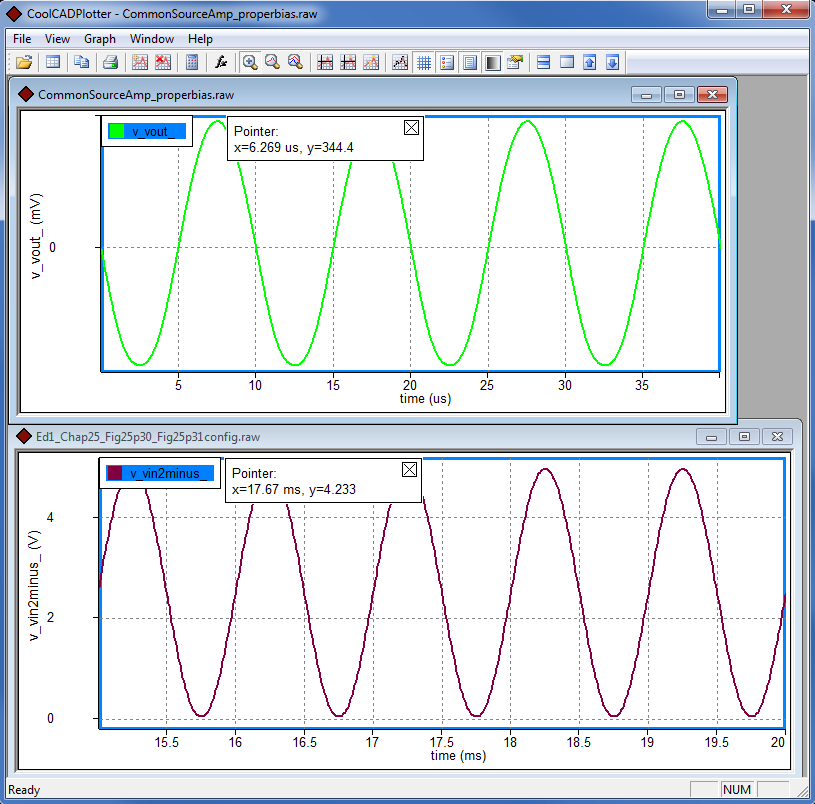
\includegraphics[width=0.6\textwidth]{./figures/plotter_netlist_editor_figures/Plotter_MultipleSubwindows.png}
    \caption{{Signals from two designs plotted in the same main Plotter window.}}
  \label{fig_plotter_multiplesubwindows}
\end{SCfigure}

\subsection{Adding Panes and Traces, Editing Traces}
\label{subsec_pane_addingtraces}

The Plotter window can be subdivided into multiple ``view"s and each "view" can be further subdivided into multiple panes. Each pane can be used to plot one or more traces. To split a pane and create a new pane, use the \textsf{Split Pane} button (see Fig. \ref{fig_plotter_multipaneaddtrace} and the annotated figures in Section \ref{subsec_pane_plotterguireference}) or the \menuitem{View}{Split Pane}. The active pane is highlighted with a blue border as shown in the figure.  Operations such as adding and removing traces are performed in the active pane, which can be selected by left-clicking in the pane area.   

\begin{SCfigure}[5.0][hbt]
    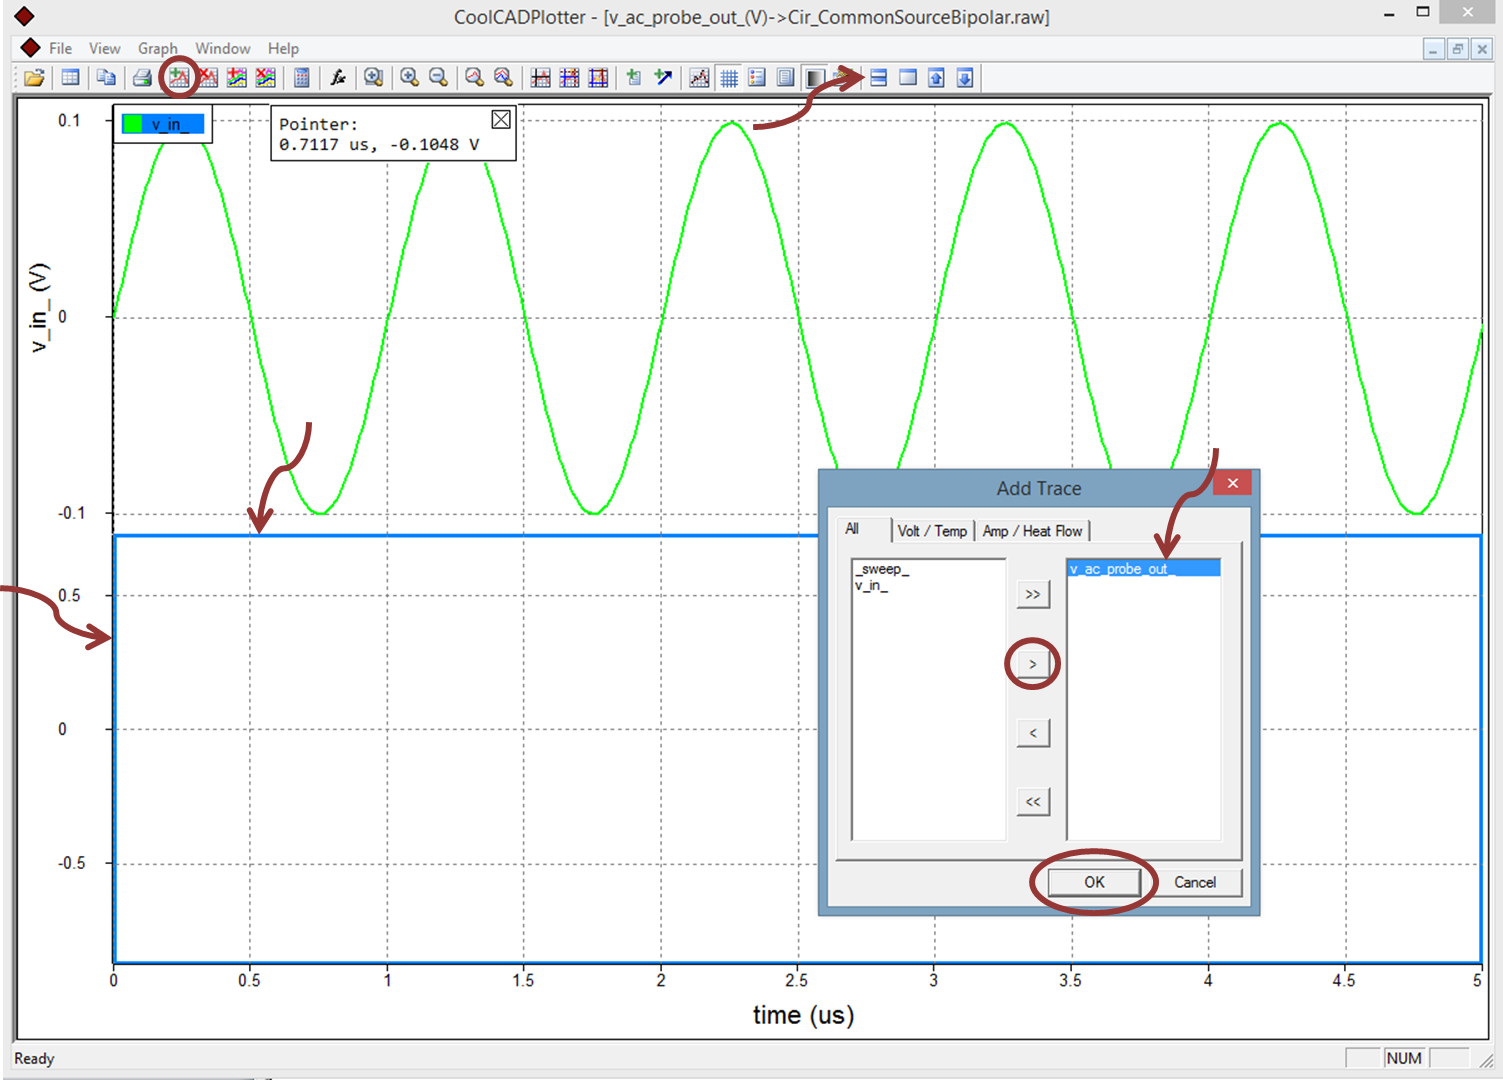
\includegraphics[width=0.6\textwidth]{./figures/plotter_netlist_editor_figures/Plotter_AddingTraces_MultiPane.png}
    \caption{{Two panes created on a plot window in which the file \textsf{Cir\_CommonSourceBipolar.raw} has been loaded.  The trace \textsf{v\_vin\_} has already been plotted on the top trace.  The bottom trace is the currently active one, into which the user is adding \textsf{v\_ac\_probe\_out\_} to plot.  The Add Trace and Split View buttons are marked by a circle and an arrow, respectively.}}
  \label{fig_plotter_multipaneaddtrace}
\end{SCfigure}

To add a trace, use the ``Add Trace" button from the button panel (see Fig. \ref{fig_plotter_multipaneaddtrace} and the annotated figures in Section \ref{subsec_pane_plotterguireference}), the \menuitem{Graph}{Add Traces}, or right-click on the active panel and choose \textsf{Add New Trace} from the contextual menu. A list of the saved traces from the loaded rawfile (or from the recent simulation, if the Plotter was initiated from a simulation) comes up. To add one or more traces select available traces from the left hand list and move them to the right hand list, when the desired traces have been selected click the \makebutton{OK} button (see \ref{fig_plotter_multipletraceadd}). 

\inserttip{If the traces chosen have different units, \textit{i.e.} if voltages and currents are chosen together, the Plotter will automatically split the view to put them on different y-axes.} 

\inserttip{The "sweep" trace is the independent variable against which the other traces are plotted.}

\begin{SCfigure}[5.0][hbt]
    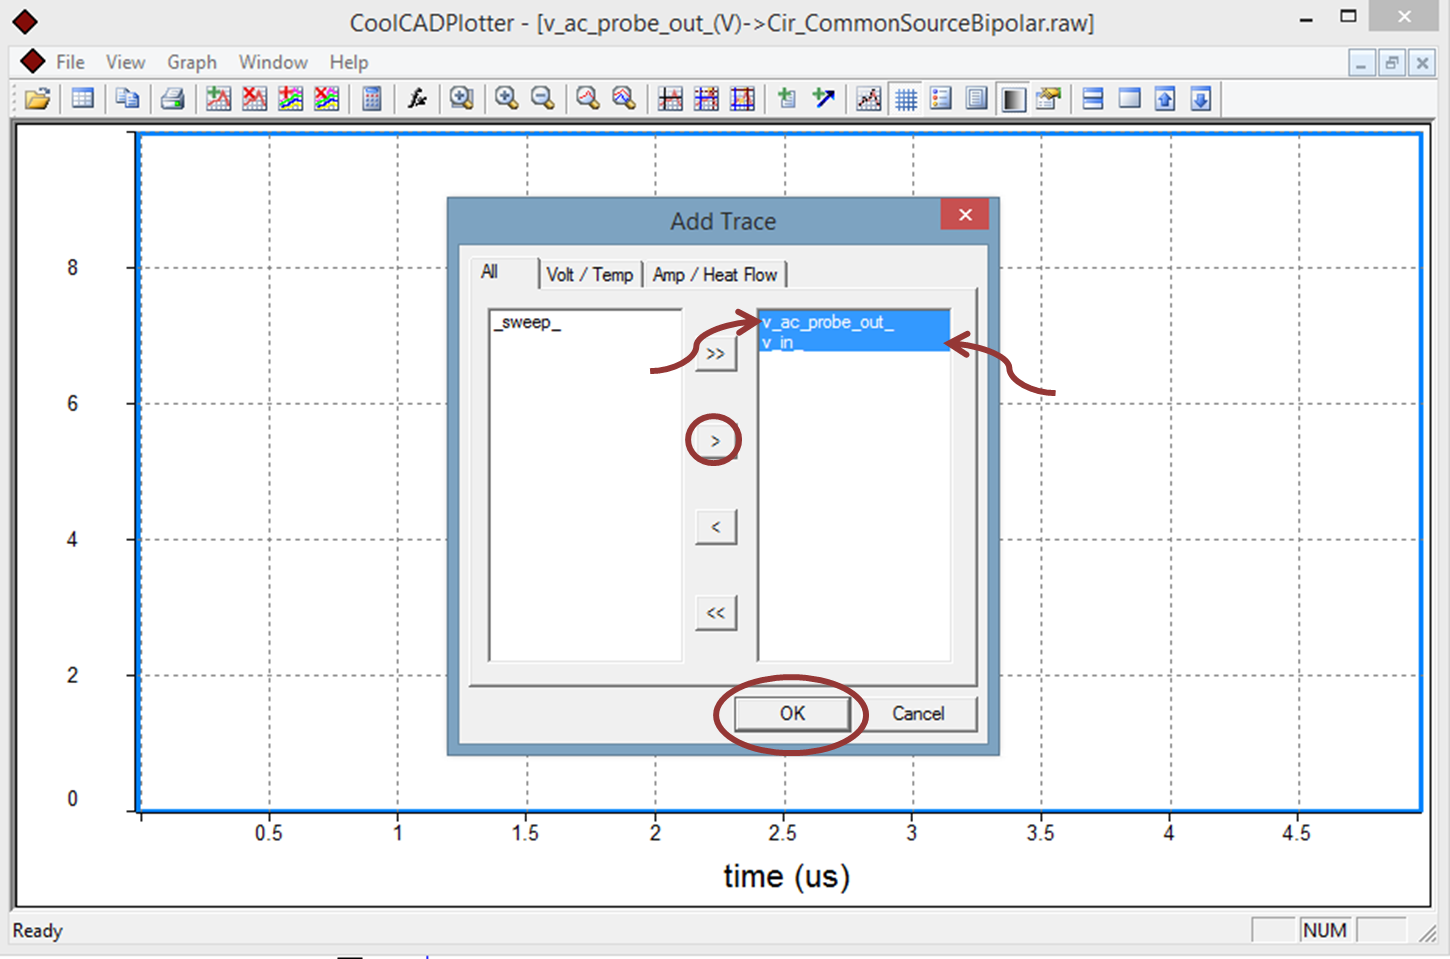
\includegraphics[width=0.6\textwidth]{./figures/plotter_netlist_editor_figures/Plotter_AddingTraces_SinglePanel.png}
    \caption{{Choosing multiple traces to plot.}}
  \label{fig_plotter_multipletraceadd}
\end{SCfigure}

\mymarginnote{Legend and pointer boxes} On each pane, by default there is a legend box which lists the traces and a trace info box, as shown in Figure \ref{fig_plotter_legendpointerboxes_traceprops}. The legend box can be toggled on/off by using the button indicated in the figure by a single dot, from the right-click contextual menu by checking ``\textsf{Show Legend}," or from the \menuitem{Graph}{Show Legend}. The trace info box can be toggled on/off by the toolbar button indicated by double dots, or from the right-click contextual menu by checking ``\textsf{Show Trace Info}." Both boxes can be moved around in the pane, so that they do not block the traces, by left-clicking within the box and dragging.

The name of the active trace is highlighted in blue in the legend box, and operations such as moving the traces between panes or deletion will be applied to the active trace (see Sec. \ref{subsec_pane_navigation}). \mymarginnote{Trace\\properties} Right-clicking within the trace info box, using the \menuitem{Graph}{Properties} or right-clicking within the pane area to bring up the contextual menu and choosing \textsf{Properties} will bring up the dialogue box which can be used to set the trace properties as shown in Fig. \ref{fig_plotter_legendpointerboxes_traceprops}. The user selects which trace to edit in the ``\textsf{Trace}" drop-down box, which lists all the invoking pane's traces and their colors. This drop down list is editable allowing renaming of the selected trace. The ``\textsf{Style}" drop-down box is used to pick the line style, choosing between solid, dashed and dotted lines. The ``\textsf{Thickness}" text box allows sets the width of the trace. The ``\textsf{Pane}" drop down list sets which pane the selected trace is in and can be used to move the trace between panes or to a newly created pane. ``\textsf{Unit}" drop down list can set the unit of the selected trace, note this will move the trace to a pane of that unit type, or a new pane if none already exists. The ``\textsf{Unit}" drop down list is editable. The color of the trace is modified with the \makebutton{Color} button.  The \makebutton{Hide} button can hide a given trace; if this option is selected and applied with the \makebutton{OK} button, the button will show up as \makebutton{Show} the next time the \window{Graph Properties} window is invoked to toggle the visibility of the trace back on. Changes made to a trace only take effect when the \makebutton{OK} button is clicked OR when a different trace is selected.

\begin{SCfigure}[5.0][hbt]
    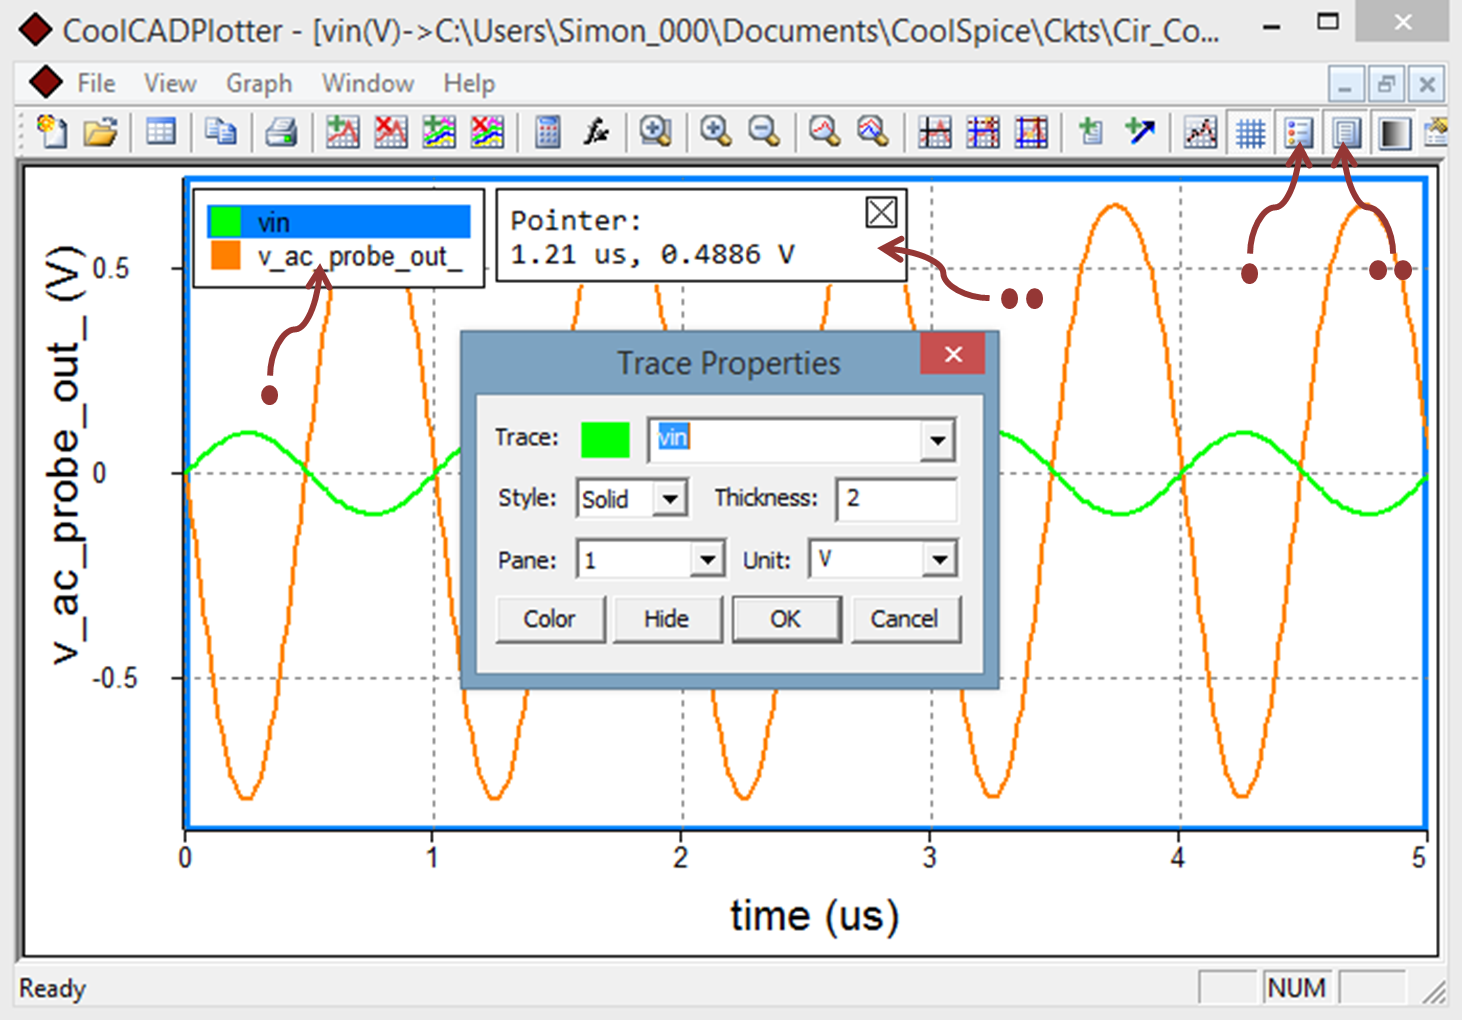
\includegraphics[width=0.6\textwidth]{./figures/plotter_netlist_editor_figures/Plotter_Legend_Pointer_Properties_Boxes.png}
    \caption{{The Trace Info box, the pointer box, and the \window{Graph Properties} dialogue window.}}
  \label{fig_plotter_legendpointerboxes_traceprops}
\end{SCfigure}

\mymarginnote{Removing\\panes} Panes can be removed or merged back into a single pane by using the ``Remove Split View" button (see Fig. \ref{fig_plotter_rightbuttons_inchapter}) or using the \menuitem{View}{Remove Split}.  All the traces present in the merged panes will be plotted in the new joint pane (assuming they have the same x-axis) and the default zoom level will fit all traces.


\subsection{Navigation}
\label{subsec_pane_navigation}

\mymarginnote{Moving traces between\\panes or\\windows} Once an active trace is selected, it can be moved between panes by either using the relevant buttons on the right-hand side of the button pane (See \ref{fig_plotter_rightbuttons_inchapter}) or the \menuitem{View}{Move Graph Up/Down}s. If multiple subwindows (with trace sets from different rawfiles) are open (as in Fig. \ref{fig_plotter_multiplesubwindows}), the active trace may be moved to one of the other subwindows by the contextual menu option ``\textsf{Move Trace to New Window}."

\newpage

\mymarginnote{Panning and zooming} Right-clicking and dragging in a pane will pan around.  If there are multiple panes sharing the same x-axis, the x-dimension panning will be mutual. The y-direction panning is always independent. Zoom-Select mode will adjust the pane to show the selected rectangle. To zoom out so that the axes span the whole of the full range of the active trace, use the ``Fit Current" toolbar button (Fig. \ref{fig_plotter_leftbuttons_inchapter}) or the \menuitem{Graph}{Zoom to Current Trace}.  To zoom out to cover the full range of all traces in the active pane, use the ``Fit All" toolbar button, or the \menuitem{Graph}{Zoom to Fit}.

\mymarginnote{Setting axis range and properties} Left-click in the area of an axis where numbers are displayed to edit the axis properties. The \window{Edit Axis} window will appear, as shown in Fig. \ref{fig_plotter_axisproperties}. The axis label, unit and minimum/maximum range can be specified with the dialog's text boxes. The user can select between linear, logarithmic and decibel modes of axis display. The user can also choose to either place ticks at a given step separation by choosing the checkbox next to \textsf{Step} and entering the separation value in the dialogue box, or the checkbox next to \textsf{Num. Ticks} and entering the desired number of axis ticks in the dialogue box.  Only one of those two options will be valid.  Finally, the axis scale can be toggled between the Plotter's automatic choice and a range of choices that make sense by using the \textsf{Scale} drop-down box.


\begin{SCfigure}[5.0][hbt]
    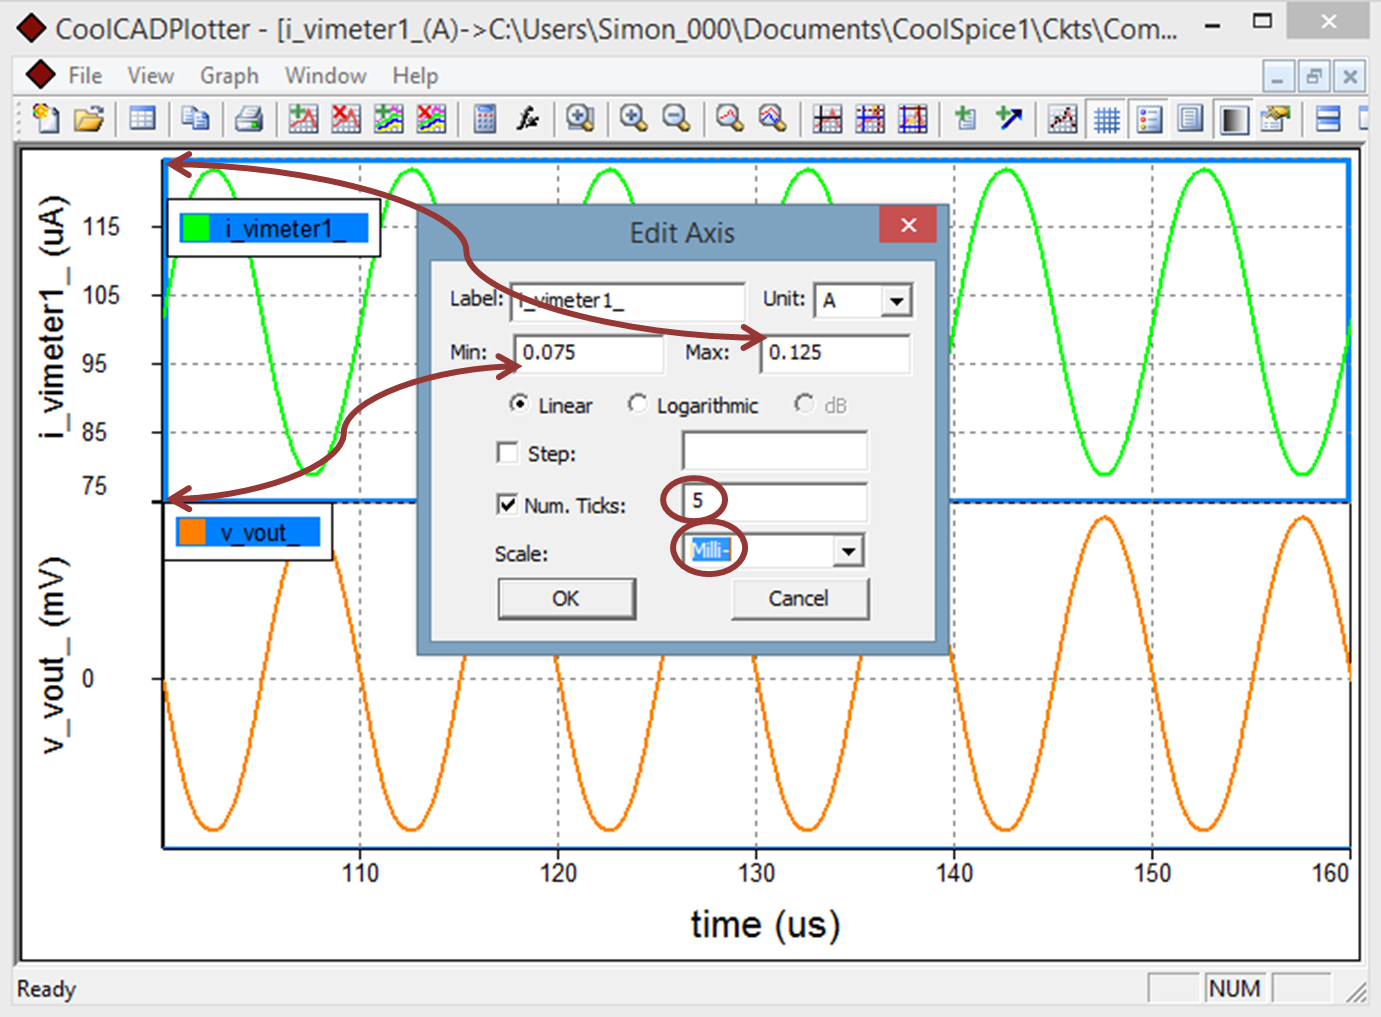
\includegraphics[width=0.6\textwidth]{./figures/plotter_netlist_editor_figures/Plotter_AxisProperties.png}
    \caption{{Setting the axis range and properties. The y-axis of the upper (active) pane has been selected in this example. The user has previously set the maximum and minimum values to 75 and 125 $\mu$A respectively, and selected the ``number of ticks" option and set five tick values to show. The scale is being set to ``milli," (which is why Min and Max are 0.075 and 0.125 in the dialog) once \makebutton{OK} is pressed, the y-axis will shift to showing the values in mA instead of the initial automatic $\mu$A choice.}}
  \label{fig_plotter_axisproperties}
\end{SCfigure}


\subsection{Measurements}
\label{subsec_pane_measurements}

The measurements can be taken on the traces are displayed in the pointer/trace info box.  

The ``\textsf{Display Difference}" toolbar button or the \menuitem{Graph}{Get Difference from Point} menu item allows the user to select a point and displays the mouse marker's difference on the trace from this point.  When this button is pressed or command selected, cursor markers appear.  Even though the intersection of the horizontal and vertical marker does not seem to be attached to the trace and can move freely around the active pane, when the user clicks the left mouse button, the point on the active trace that corresponds to the that x-axis location is marked and shown as ``\textsf{Cursor 1}" in the pointer box. After this point, a new pair of horizontal/vertical cursor lines, shown as the ``\textsf{Cursor 2}" location in the pointer box, are invoked and are attached to the active trace.  As the user moves the mouse around, the cursor lines for Cursor 2 move along the trace and the x-axis and y-axis distances of the real-time location from the previously-marked point are displayed in the pointer box as \textsf{dx} and \textsf{dy}, as shown in Fig. \ref{fig_plotter_distancefrompoint}.  

If the trace is a time-domain signal, the pointer box also shows ``\textsf{freq}", which is 1/\textsf{dx}.

\begin{SCfigure}[5.0][hbt]
    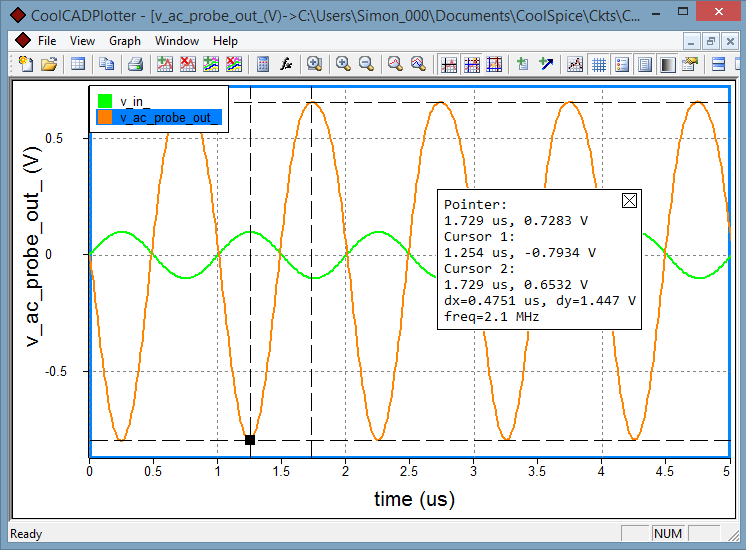
\includegraphics[width=0.6\textwidth]{./figures/plotter_netlist_editor_figures/Plotter_DisplayDifference.png} %Plotter_DifferencefromaPoint_Measurement
    \caption{{Measurement from a point.  In this example, the point \nobreak{$(x,y)=(1.254$ $\mu$s,} -0.7934 V) has been selected and the mouse pointer (not visible) has been moved to \nobreak{$(x,y)=(1.729$ $\mu$s, 0.7284 V),} which puts the trace-attached Cursor 2 at \nobreak{$(x,y)=(1.729$ $\mu$s}, 0.6532 V).  \nobreak{$\Delta x$=\textsf{dx}=0.4751 $\mu$s,} \nobreak{$\Delta y$=\textsf{dy}=1.447 V.}}}
  \label{fig_plotter_distancefrompoint}
\end{SCfigure}

The ``\textsf{Get Difference Between Points}" button (See Fig. \ref{fig_plotter_rightbuttons_inchapter} for the button marked ``Two Selected Points Diff" or the \menuitem{Graph}{Get Difference between Points}) works the same way. However, this option allows the user to mark first the point for Cursor 1, then the point for Cursor 2, and then turns off the cursors.  To select new points, the user has to toggle the menu option off and back on.  Once the option is turned off, the marked points and the difference value display in the pointer box will disappear.

\subsection{Calculator}
\label{subsec_pane_calculator}

The calculator can be invoked by the Calculator button (see Fig. \ref{fig_plotter_leftbuttons_inchapter}) or the \menuitem{Graph}{Calculator}.  The traces present in the loaded rawfile are available as data items, effectively vectors, in the calculator.  Calculations can be carried out using numbers and functions just as in a regular calculator. Expressions can be generated using the buttons or manually entered into the Expression text box. For calculations which evaluate to a single number, clicking the \makebutton{Eval} button evaluates the expression and puts the result in the calculator's Expression text box.  For these calculations, using the \makebutton{Graph} button graphs a constant value vs. the same x-axis as the active trace. For expressions which must evaluate to a trace, the \makebutton{Eval} button has no function. The \makebutton{Graph} button graphs the calculated variable in the active pane if the y-axis is compatible, or in a new pane if necessary. To select the trace or traces to use as a variable, the user can either enter the trace names exactly as shown in the selection box into the Expression text box, or simply click on the name of the trace in this box, which will then copy the name over to the expression box, as shown in Fig. \ref{fig_plotter_usingcalculator}. Multiple expressions can be graphed simultaneously by separating them with a comma. A unit can be specified in the editable Unit drop down menu, this allows the user to control the destination pane for the graphed expression. A trace name can be specified in the Trace name text box to be used as a name for the graphed trace in place of the expression itself, multiple names can be specified for multiple traces separated by commas.

\begin{SCfigure}[5.0][hbt]
    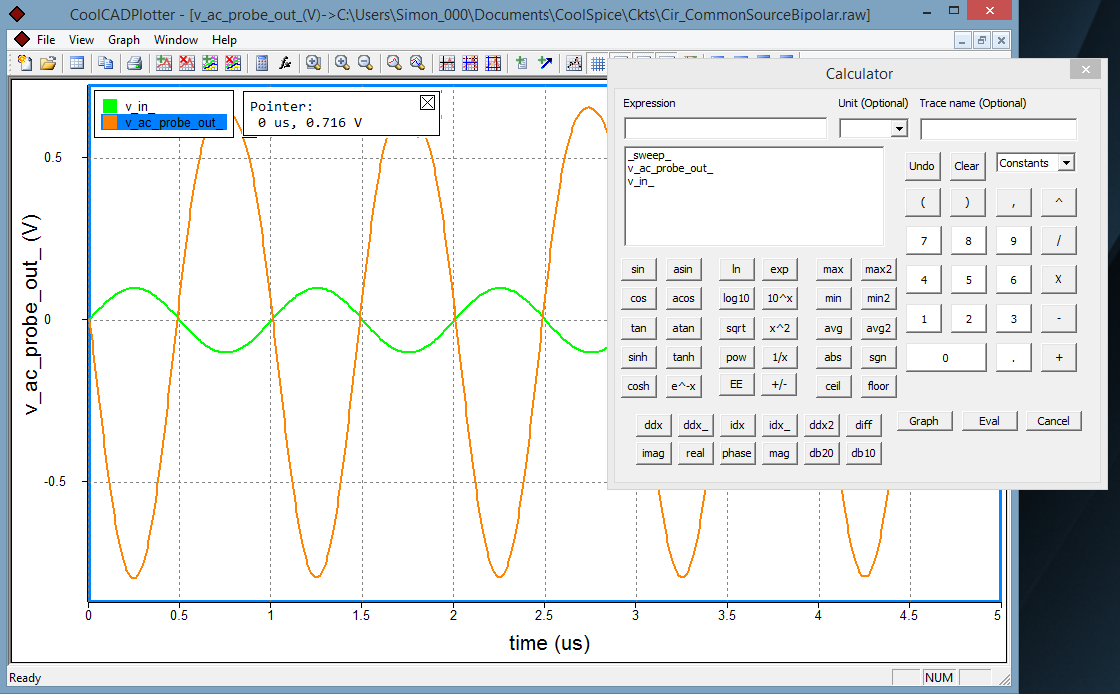
\includegraphics[width=0.6\textwidth]
		{./figures/plotter_netlist_editor_figures/Plotter_Calculator.png} %Plotter_Calculator_1
    \caption{{The calculator showing available traces.}}
  \label{fig_plotter_usingcalculator}
\end{SCfigure}

\subsection{Plotter Options and the Contextual Menu}
\label{subsec_pane_plotteroptions}

The display options of the Plotter, which can be accessed through the \textsf{\textbf{Graph}} menu or the contextual menu and toggled on or off by clicking on them, are as follows:
\begin{itemize}
\item \textsf{\textbf{Show Data Points}}: By default, the Plotter interpolates between the data points saved in the rawfile when plotting a trace.  When this option is toggled on, individual data points are marked on the curve.
\item \textsf{\textbf{Show Grid}}: Toggle on/off the grid display.
\item \textsf{\textbf{Show Legend}}: Toggle on/off the trace legend box display in the active pane.
\item \textsf{\textbf{Show Trace Info}}: Toggle on/off the pointer/trace information box display in the active pane.
\item \textsf{\textbf{White Background}}: Switch between white and dark backgrounds.
\end{itemize}

\mymarginnote{The contextual menu}The contextual menu is invoked by right-clicking anywhere within the panes.  Figure \ref{fig_plotter_contextualmenu} shows the menu items, some of which are toggle options.

\begin{SCfigure}[5.0][hbt]
    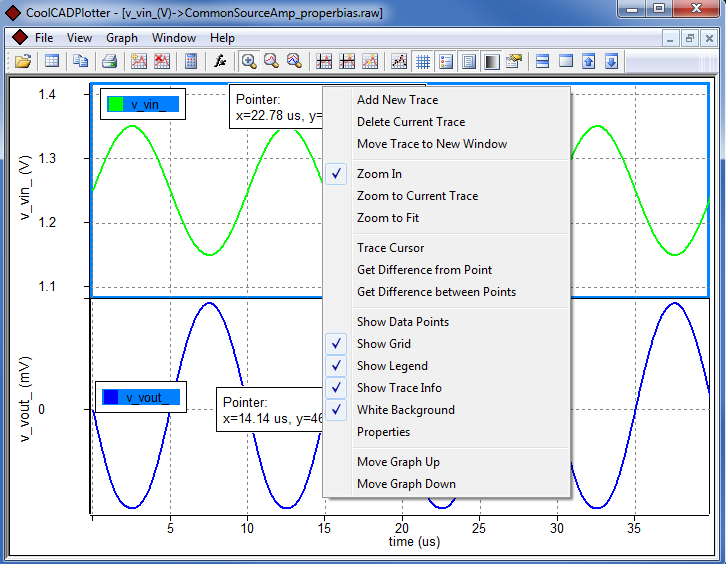
\includegraphics[width=0.6\textwidth]{./figures/plotter_netlist_editor_figures/Plotter_ContextualMenu.png}
    \caption{{The contextual menu items.}}
  \label{fig_plotter_contextualmenu}
\end{SCfigure}

The contextual menu items are as follows:
\begin{itemize}
\item \textsf{Add New Trace} and \textsf{Delete Current Trace} bring up the dialog box to plot new trace or traces, and delete the active trace, respectively.
\item \textsf{Move Trace to New Window} moves the active trace to another subwindow, as described in Sec. \ref{subsec_pane_navigation}.
\item \textsf{Zoom In, Zoom to Current Trace} and \textsf{Zoom to Fit} are zooming options described in Sec. \ref{subsec_pane_navigation}.
\item \textsf{Trace Cursor} is a toggle option which turns on/off dashed cursors to indicate the pointer location in the pane.
\item \textsf{Get Difference from Point} and \textsf{Get Difference between Points} are used to perform measurements on the traces as described in Sec. \ref{subsec_pane_measurements}.
\item \textsf{Show Data Points} is a toggle option which shows/hides data points that were saved in the rawfile. The \menuitem{Graph}{Show Point Marks} has the same function. 
\item \textsf{Show Grid} is a toggle option to turn on/off the grid. The \menuitem{Graph}{Show Grid} has the same function.
\item \textsf{Show Legend} and \textsf{Show Trace Info} are toggle options which display/hide the legend box and the pointer box, respectively.  The \menuitem{Graph}{Show Legend} has the same function for the former.
\item \textsf{White Background} is a toggle option which makes the background white or black.  The \menuitem{Graph}{Use White Background} has the same function.
\item \textsf{Properties} brings up the \window{Graph Properties}.
\item \textsf{Move Graph Up/Down} items move the traces between panes.
\end{itemize}



\subsection{Plotter GUI Reference}
\label{subsec_pane_plotterguireference}

See Appendix section for larger versions of these images.

\begin{SCfigure}[5.0][h]
    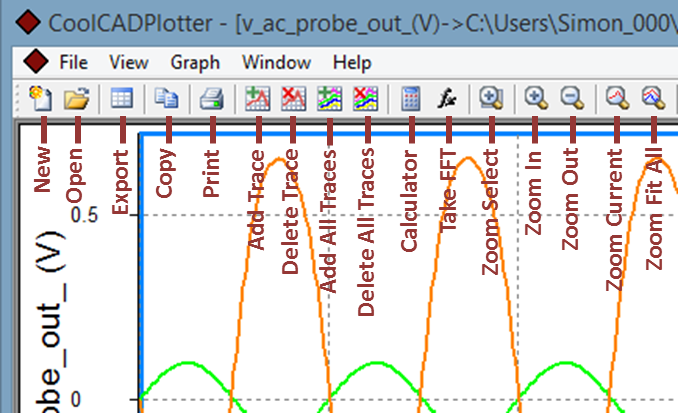
\includegraphics[width=0.45\textwidth]{./figures/appendix_buttons_menus_figures/Plotter_LeftButtons.png}
    \caption{{Left-side buttons on the Plotter.}}
  \label{fig_plotter_leftbuttons_inchapter}
\end{SCfigure} 

\begin{SCfigure}[5.0][h]
    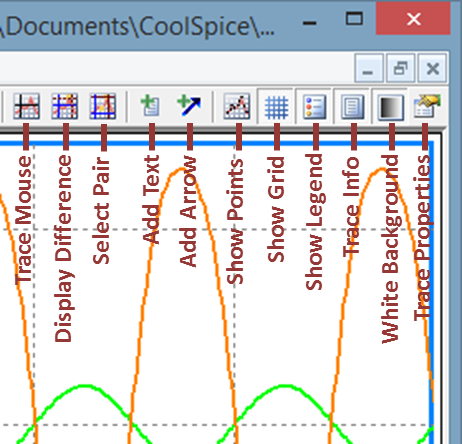
\includegraphics[width=0.45\textwidth]{./figures/appendix_buttons_menus_figures/Plotter_RightButtons.png}
    \caption{{Right-side buttons on the Plotter.}}
  \label{fig_plotter_rightbuttons_inchapter}
\end{SCfigure} 

A list of menu items for the Plotter can be found in the Appendix Section.

\section{Netlist Editor}
\label{sec_pane_netlisteditor}

\subsection{SPICE Netlist Syntax}
\label{subsec_pane_spicenetlistsyntax}

All SPICE commands, including analysis commands, begin with ``.", such as ``\texttt{.include}", ``\texttt{.tran}", or ``\texttt{.end}".  Component descriptions begin with a single character indicating the type of the component, such as \texttt{M} for MOSFETs, \texttt{D} for diodes and \texttt{R} for resistors.  

\mymarginnote{Beginning \\and ending} The first line of any SPICE file must be a commented title line starting with '*'.  The last line of any SPICE file must be an \texttt{.end} statement: 

\spicesyntax{.end}

\mymarginnote{Commenting} The comment character is '*' and is placed at the beginning of a line. For example, in the following code snippet, the first and third lines are comments:

\spicesyntax{\begin{tabular}{ll}
&* Trying two resistor values by commenting one out at a time \\
&R12 N2 N3 40k \\
&*R12 N2 N3 60k \\
&C12 N2 N3 10p
\end{tabular}
}

Multiple lines can commented and uncommented \makekey{CTRL}-\makekey{K} and \makekey{CTRL}-\makekey{SHIFT}-\makekey{K}, useful for disabling and enabling blocks of the netlist.\\


\mymarginnote{Multi-line \\ statements} When a statement continues for more than a single line in the text file, the \texttt{+} character must be used to indicate the new line is a continuation of the previous statement. For instance:

\spicesyntax{\begin{tabular}{ll}
&.model newpmos pmos ( LEVEL   = 49 \\
&+VERSION = 3.1  TNOM = 27  TOX = 1.4E-8 XJ = 1.5E-7 NCH = 1.75E17  \\
&+VTH0 = -0.9 K1 = 0.55	K2 = 8E-3  K3 = 1.5  K3B = 0.025  W0 = 1E-8 \\
&+(...)
\end{tabular}}


\mymarginnote{The \texttt{.include} statement} The \texttt{.include} statement is used to include subcircuit and device model definitions from another text file containing \texttt{.subckt} and \texttt{.model} statements. For long, complicated circuits, this allows the user to keep the main circuit topography, simulation options and simulation commands in one file while keeping the device and subcircuit definitions in auxiliary files.  For example, 

\spicesyntax{\begin{tabular}{l}
* Schematics Netlist * \\
.include "../Models/MyMOS.txt" \\
\\ 
MN1\_x line\_out \_HN\_1\_Vin 0 0 nmos0p5 W=3u L=0.6u \\
MP1\_x line\_out \_HN\_1\_Vin \_HN\_1\_VDD \_HN\_1\_VDD pmos0p5 W=4.5u L=0.6u \\
VVG1 \_HN\_1\_Vin 0   DC  3         \\
VVS1 VDD 0   DC  3     \\
\\
.dc VVG1 0 3 0.05   \\
.end 
\end{tabular} }
 
In this example, the models \texttt{nmos0p5} and \texttt{pmos0p5} must be defined in the file \textsf{../Models/MyMOS.txt}. More details about the \texttt{.include} statement can be found elsewhere.  

The \texttt{.subckt} statement is used to define a subcircuit, \mymarginnote{The \texttt{.subckt} statement} which acts like a device model which incorporates other device models. Once defined, multiple instances of the subcircuit can then be invoked  throughout the main circuit just as the case for a regular device. Parameters defined within a subcircuit are visible only within the scope of that subcircuit, and if two parameters of the same name exist within nested scopes the parameter of the smaller scope is utilized. Subcircuits can be nested.


\subsection{Editing and Running a Netlist}
\label{subsec_pane_editingrunningnetlist}

To run the Netlist Editor, click on the \textsf{Netlist Editor} button on the CoolSPICE main console window.

\menuitem{File}{New}, \makebutton{New} toolbar button or \makekey{CTRL}-\makekey{N} will open a new, empty file. A SPICE netlist can simply be typed in and saved by \menuitem{File}{Save} or \makekey{CTRL}-\makekey{S}.  For the syntax, see Section \ref{subsec_pane_spicenetlistsyntax} above.  

More often, an existing netlist generated by the Schematic Editor is opened to be edited by \menuitem{File}{Open} or \makekey{CTRL}-\makekey{O}.  Figure \ref{fig_netlisteditor_netlistexample1} shows an example circuit and its netlist opened in the Netlist Editor after being generated by the Schematic Editor.  It is possible to save an open netlist under another name with the \menuitem{File}{Save As} or \makekey{CTRL}-\makekey{SHIFT}-\makekey{N}.

\begin{figure}[bh]
  \centering
    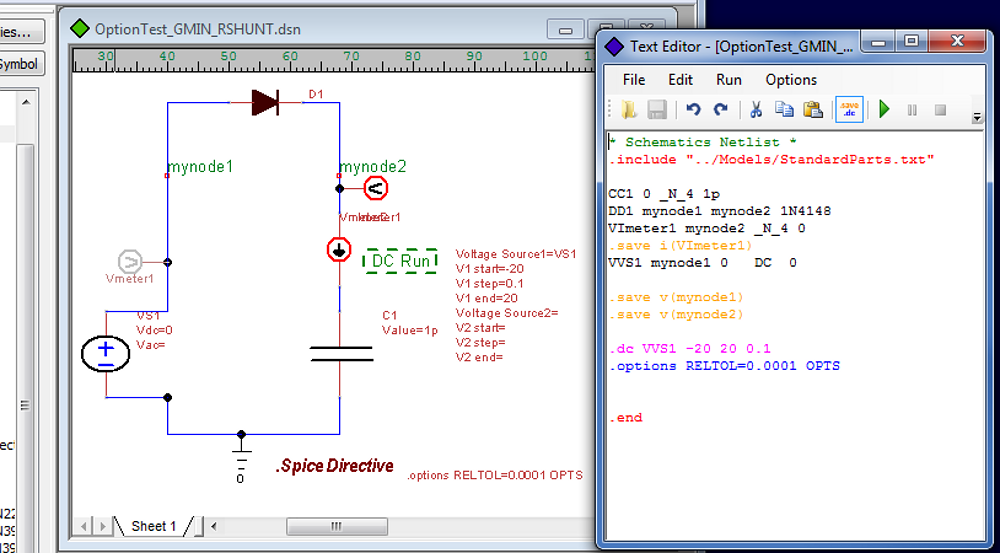
\includegraphics[width=0.8\textwidth]{./figures/plotter_netlist_editor_figures/NetlistEditor_ExampleNetlist1.png}
    \caption{An example circuit open in the Schematic Editor and the corresponding netlist open in the Netlist Editor (the window is named ``Text Editor").}
  \label{fig_netlisteditor_netlistexample1}
\end{figure} 

To run the SPICE netlist, press \makekey{F5}, use the \menuitem{Run}{Run Netlist}, or press the ``Play" button.  The progress bar will display the progress of the simulation.  Long simulations can be paused by the ``Pause" button or stopped by the ``Stop" button.  See Sec. \ref{subsec_pane_netlisteditorguireference} for an annotated screenshot showing the button locations.

\subsection{Netlist Editor Options}
\label{subsec_pane_netlisteditoroptions}

The options available under the \textsf{\textbf{Options}} menu are the same as those available under the \menuitem{SPICE}{Preferences} of the Schematic Editor with one exception, Syntax Highlighting. These are all toggle-on or toggle-off options.  

\textsf{\textbf{Open Plotter}}, if checked, will automatically launch the Plotter after a simulation is successfully completed.  If this option is checked but there are no plottable results (e.g. due to convergence problems or a netlist error) an error message window will show up instead.

\textsf{\textbf{Show Rawfile}}, if checked, will automatically display the raw result data of the simulation after the simulation is successfully completed.

\textsf{\textbf{Show Logfile}}, if checked, will automatically display the simulation log file after the simulation or simulation attempt is complete. Note that the log file for the most recent run of the netlist can be opened at anytime with \makekey{CTRL}-\makekey{L}.

\textsf{\textbf{Measure (No Rawfile)}} only applies to netlists containing a \texttt{.measure} statement and asks the program to look for and display only the log file output with the measurement results after the simulation is complete.

\textsf{\textbf{Highlight}}, if checked, will automatically color lines of the netlist according to their type, e.g. green for comments. Syntax Highlighting can also be toggled with \makekey{CTRL}-\makekey{H} or the Syntax Highlight toolbar button.

As a display option, the button ``Syntax Highlight On-Off" (see Section \ref{subsec_pane_netlisteditorguireference}) will turn the color-coding of the SPICE commands on or off.

\label{subsec_pane_netlisteditorguireference}

\begin{figure}[htb]
  \centering
    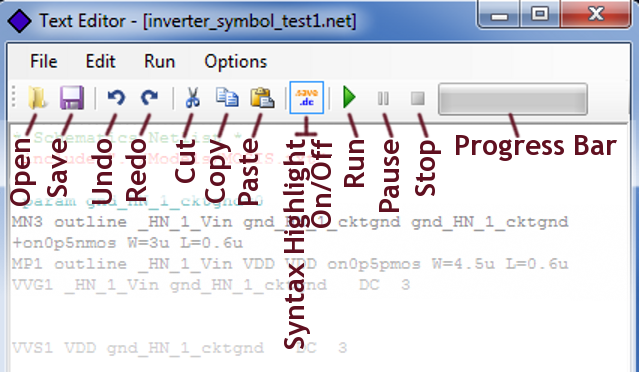
\includegraphics[width=0.8\textwidth]
		{./figures/appendix_buttons_menus_figures/NetlistEditor_AllButtons.png}
    \caption{Buttons on the Netlist Editor.}
  \label{fig_netlisteditor_allbuttons_inchapter}
\end{figure} 

A list of menu items for the Netlist Editor can be found in the Appendix Section.
